% !TeX spellcheck = en_US
\chapter{Related work}%

\section{Prior Providentia Mono3D Toolchain}

The Providentia Monocular 3D Object Detection task (Mono3D) decribes the process of detecting three-dimensional objects from a single two-dimensional RGB camera output frame. The Providentia Mono3D toolchain is described in details in the bachelor thesis “Real-Time Monocular 3D Object Detection to Support Autonomous Driving” of Leon Blumenthal \cite{thesisLeon} and the master thesis "Monocular 3D Object Detection Using HD Maps" of Joseph Birkner \cite{thesisJoseph}, both under the supervision of  M.Sc. Walter Zimmer. 

In \cite{thesisLeon}, the Providentia Mono3D detecter splits the detection task into two separate steps: a 2D instance segmentation step, and a 3D lifting step. This so-called two-stage detection model is adapted and refined in the thesis of Joseph  \cite{thesisJoseph}. The first work focused on highway senario, where the yaw value (the travel/ heading direction) is fixed. The second work covered/generalized to the more urban scenarios where the yaw value is variable. This is achieved with the proposed augmented L-Shape fitting algorithm supporting tracking and HD Map confidence inputs. The proposed approach was then evaluated on the Providentia Intersection Scenario dataset, which includes frames taken from two cameras installed at an intersection called s110 under the Providentia project, with resolution of 1920x1200 pixels and run at 60 Hz. This dataset will be covered in more detail in section 3.2. Another improvement taken place was the switch from Yolact-Edge to YOLOv7 to improve the 2D instance segmentation step. 

The pipeline of the current Providentia Mono3D Toolchain can be summarized as followed: 
\begin{itemize}
	\item The 2D object detector YOLOv7 detect objects and publish an array of detection triplets containing of category, 2D bounding box , and mask for each frame. 
	\item The instance mask's bottom contour is extracted from the 2D mask. This operation return a line of 2D pixel coordinates for each bottom contour. 
	\item The bottom contour is then projected back into 3D map space 
	\item Then the yaw value (the headling value) is selected for each 3D vehicle detection from a traffic flow direction that is derived from the HD map. (HD Map Lookup Grids are queried at the positions of the 3D points of the bottom countour.)
	\item The proposed L-Shape-Fitting (LSF) algorithm estimates the physical length and width of the bottom contour. 
	\item The object's height and position is estimated using a proposed joint height and position regression. 
	\item Finally, the 2D instance bounding box is matched against historical detections via SORT object tracking to find previous detections of the same vehicle. 
\end{itemize}


\section{TUMTraf Intersection Dataset}

The TUMTraf Intersection Dataset is the R2 release of TUMTraf dataset \cite{a9dataset}. This release was publised in June 2023 under the name "A9 Intersection Dataset" \cite{zimmer2023a9}. With two roadside cameras and LiDARs mounted on intersection gantry bridges, the dataset provides 4.8k synchronized images and LiDAR point clouds with more than 57.4k manually labeled 3D bounding boxes. The data labels are in OpenLABEL format \cite{openlabel}. \hl{Detail about OPENLabel in section 3.3.} The ten classes annotated are CAR, BUS, TRUCK, TRAILER, VAN, MOTORCYCLE, BICYCLE, PEDESTRIAN, EMERGENCY\_VEHICLE, or OTHER. 

The dataset contains four scenes of varying length (between 300 and 1200 frames) at a frame-rate of 10 Hz. The dominant class is CAR, then come the classes TRUCK, TRAILER, VAN, and PEDESTRIAN with roughly the same order of magnitude. The remaining five classes are present in a slightly smaller number. 

\hl{
- 78.2\% were classified as NOT OCCLUDED, 16.1\% as PARTIALLY OCCLUDED, 0.8\% as MOSTLY OCCLUDED, and 4.9\% were classified as UNKNOWN (not labeled)
}


\section{You Only Look Once (YOLO}

You Only Look Once (YOLO) is a SOTA object detection and image segmentation system that has revolutionized the field of computer vision. YOLO is known for simple architecture, fast inference speed and thus suited for real-time object detection tasks. YOLO was first introduced in 2015 \cite{yolo} and since then several new versions of the same model have been proposed. 

The Providentia Mono3D Detector is currently using YOLOv7 instance segmentation model.This model is YOLOv7 \cite{yolov7} fine-tuned on the MS COCO \cite{lin2014microsoft} instance segmentation dataset to leverage YOLOv7 for instance segmentation. The system detects six sub-classes of MS COCO: CAR, BUS, TRUCK, MOTORCYCLE, BICYCLE, PEDESTRIAN. The remaining three classes of TUM Traffic Datase: VAN, EMERGENCY\_VEHICLE, and OTHER  cannot yet be recognized. 

In this work, we switch from YOLOv7 to YOLOv8 to enhance detection speed and accuracy. YOLOv8 is the latest version of YOLO and introduces several new features and improvements  for enhanced performance, flexibility, and efficiency. Performance tests have shown that YOLOv8 outperforms YOLOv7 in terms of speed and accuracy. \hl{Say something about the comparison figure}

% \centering
%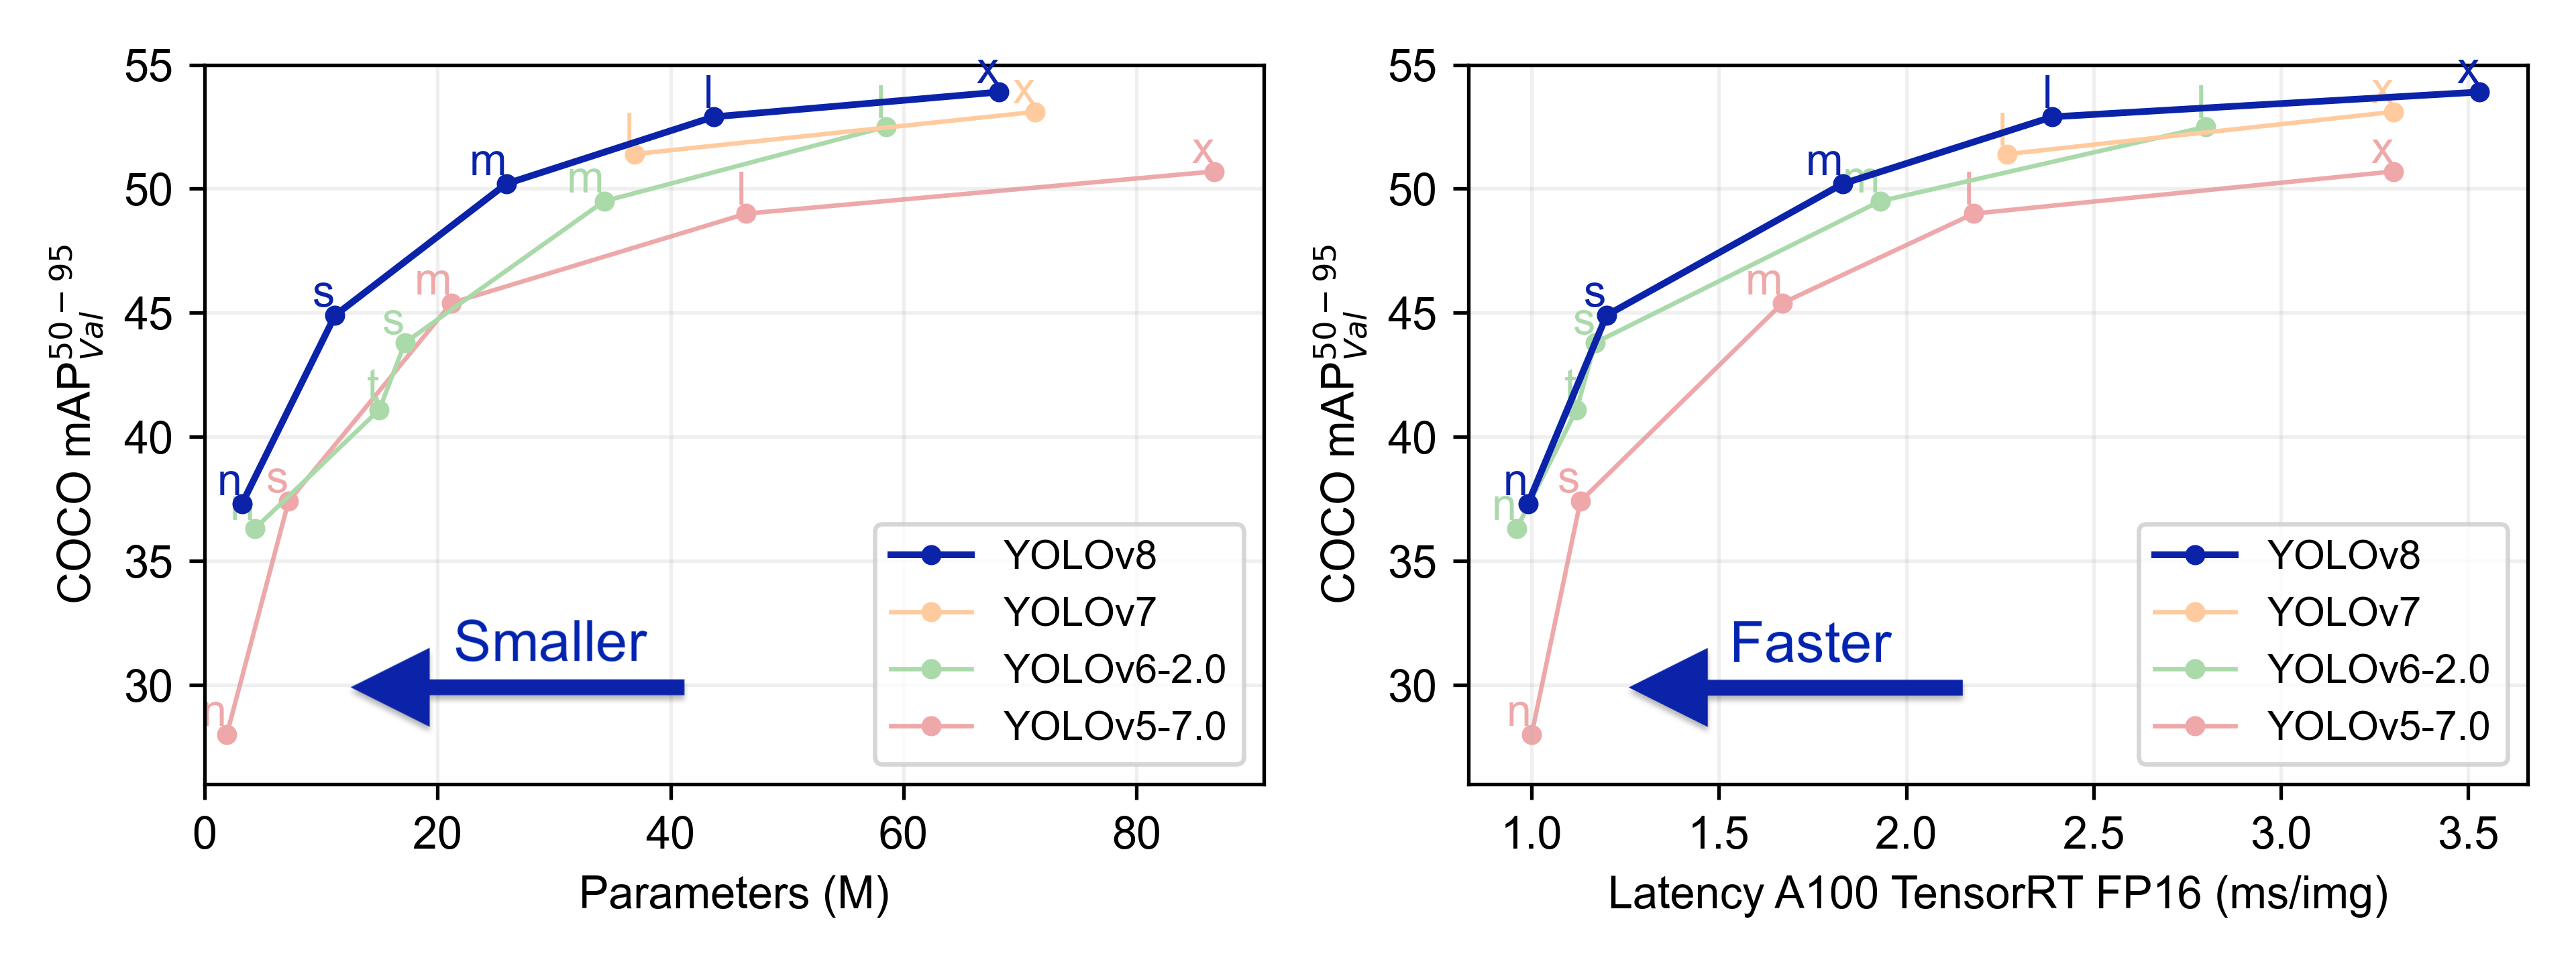
\includegraphics[width=120mm]{figures/yolo-comparison-plots.png}%

\begin{figure}[htb]%
	\centering%
	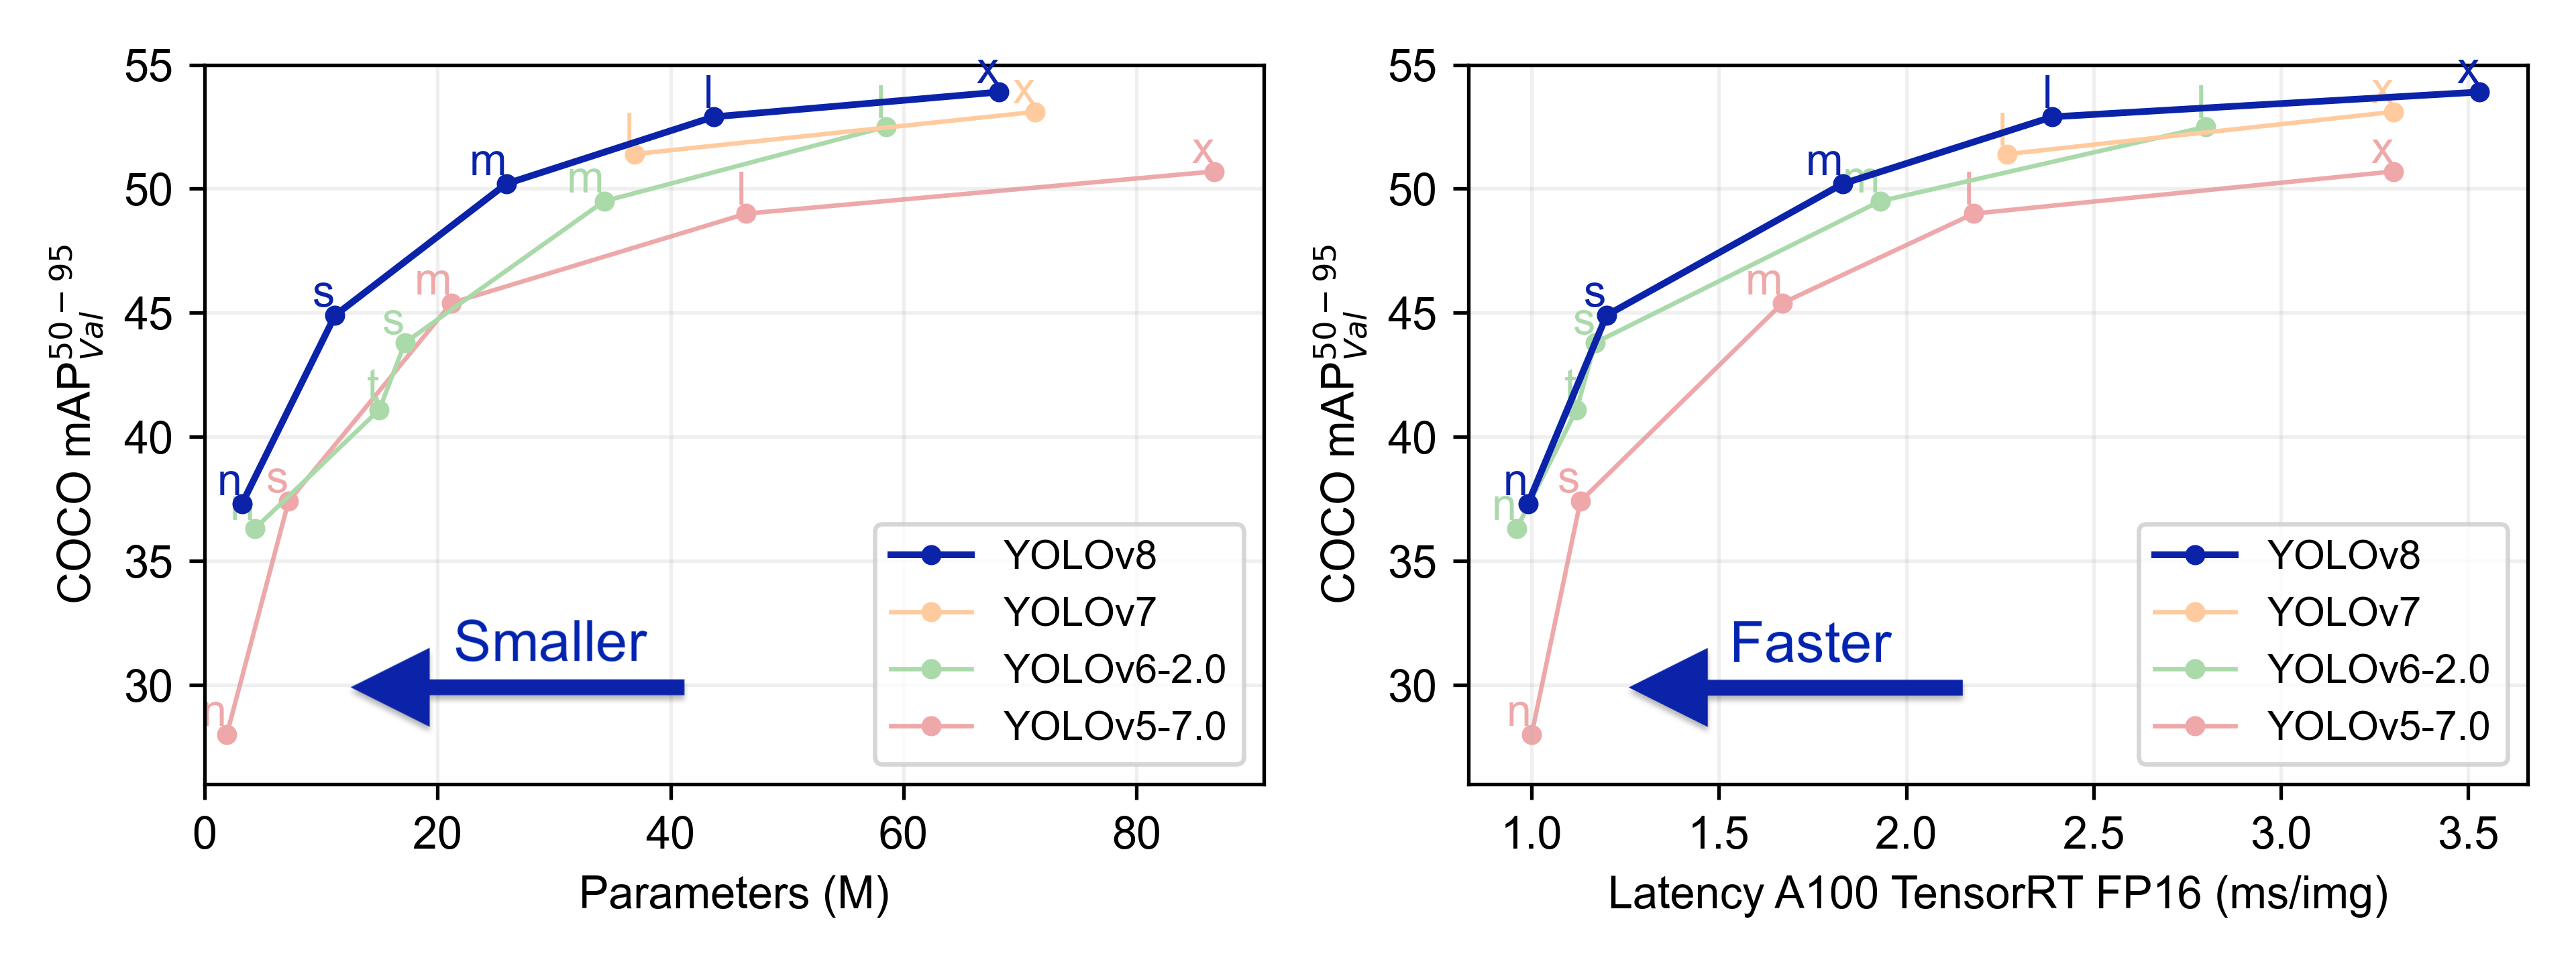
\includegraphics[width=150mm]{figures/yolo-comparison-plots.png}%
	\caption{YOLO parameters and latency comparison.}%
	\label{YOLO comparison}%
\end{figure}%

We choose the biggest model: YOLOv8x and additionally, we fine-tuned the models on our TUM Traffic dataset so that the model can detect all ten classes and improve the accuracy further. \hl{More on this in the dataset annotate and training section later.}

\subsection{TensorRT Optimization}

To preserve the real-time requirement of the Providentia system, we export the model to TensorRT to accelerate inference. NVIDIA’s TensorRT  \cite{vanholder2016efficient} is a high-performance deep-learning inference library designed to optimize and accelerate the inference of deep neural networks on NVIDIA GPUs. 

\section{C2F Seg}
\hl{TODO. Optional, if talk about C2F later}


\section{Annotation/Label Format}

- general description. Which formats will be presented. Which dataset use these formats? 
- we extended the TUMTraf dev-kit with label converters between these three format YOLO, COCO, OPENLabel. 

\subsection{OPENLabel Format}

The Association for Standardization of Automation and Measuring Systems (ASAM) with Deepen AI released the OpenLABEL  \cite{openlabel}, a standard designed to specify an annotation format flexible enough to support the development of automated driving features and to guarantee interoperability among different systems and providers. JSON schema is used to define the annotation structure of OpenLABEL and therefore annotation files are stored in .json format. 

TUMTraf dataset fully adopted this OPENLabel annotation format. \hl{Describe the TUMTraf annotation format with poly2d, bbox in with full and visible?}

\subsection{YOLO Format}

\subsection{COCO Format}
-  The annotations are stored using JSON.

\begin{mdframed}
	\textbf{COCO Annotation Format:}
	\begin{verbatim}
		{
			"annotation": {
				"id": int,
				"image_id": int,
				"category_id": int,
				"segmentation": RLE or [polygon],
				"area": float,
				"bbox": [x,y,width,height],
				"iscrowd": 0 or 1
			},
			"categories": [
			{
				"id": int,
				"name": str,
				"supercategory": str
			}
			]
		}
	\end{verbatim}
\end{mdframed}

%\begin{lstlisting}[caption={COCO Annotation Format}]
%	{
%		"annotation": {
%			"id": int,
%			"image_id": int,
%			"category_id": int,
%			"segmentation": RLE or [polygon],
%			"area": float,
%			"bbox": [x,y,width,height],
%			"iscrowd": 0 or 1
%		},
%		"categories": [
%		{
%			"id": int,
%			"name": str,
%			"supercategory": str
%		}
%		]
%	}
%\end{lstlisting}

\section{CVAT Labelling Tool}

To extend the TUMTraf Intersection Dataset with visible and full instance masks annotation, we use the open-source annotation tools CVAT (Computer Vision Annotation Tool) \cite{cvat} developed by Intel. 

Benefits: 
- CVAT allows users to annotate images with four types of shapes: boxes, polygons, polylines, and points. 
- CVAT supports multiple annotation formats including YOLO, MS COCO Object Detection, KITTI and many more. 
- CVAT supports automatic labeling by exploiting serverless deep learning model such as YOLO, RCNN, Face Detection, Segment Anything and many more. 

